\documentclass[12pt]{article}
\usepackage{style}
\begin{document}
\backgroundsetup{contents={}}
\section{Assignment 1}
\begin{enumerate}
    \item Define streamline and path line. Derive the equation of continuity for the motion of a compressible fluid. Show that if the fluid is incompressible and the motion is irrotational then it can be expressed as $ \nabla^2 \phi=0 $, where $ \phi $ is the velocity potential.
    \item Derive the differential equation of streamline and path line. When do the streamline and path line coincides?
    \item State and proof Bernoulli's theorem for steady motion of an inviscid fluid. Hence, derive Bernoulli's theorem for barotropic flow. 
    \item Show that the variable ellipsoid 
    \[
        \frac{x^2}{a^2k^2t^4}+kt^2\left\{ \left( \frac{y}{b} \right)^2+\left( \frac{z}{c} \right)^2 \right\}=1,
    \]
    is a possible form of boundary surface of a liquid at any time $ t $.
    \item Derive the equation of motion for incompressible inviscid fluid in the form $ \frac{\mathrm{d}\bar{q}}{\mathrm{d}t}=\bar{F}-\frac{1}{\rho}\nabla p $.
    \item Show that, $ u=\frac{2xyz}{\left( x^2+y^2 \right)^2}, v=\frac{\left( x^2-y^2  \right)z}{\left( x^2+y^2 \right)^2} $ and $ w=\frac{y}{x^2+y^2} $ are the velocity components of a possible fluid motion.
    \item Derive streaming motion past a circular cylinder.
    \item Define source, sink and doublet. Determine the complex potential foe a doublet of stream $ \mu $, placed at the point $ z=a $ which makes an angle $ \alpha $ with positive $ x- $axis.
\end{enumerate}
\newpage
\begin{prob}
    Define streamline and path line. Derive the equation of continuity for the motion of a compressible fluid. Show that if the fluid is incompressible and the motion is irrotational then it can be expressed as $ \nabla^2 \phi=0 $, where $ \phi $ is the velocity potential.
\end{prob}
\begin{soln}
    \emph{Streamline:} A line drawn in the fluid so that its tangent at each point is in the direction of the fluid velocity at that point is called a streamline.

    
    \emph{Path line:} The curve which a particular particle of the fluid describes during its motion is called a path line.

    \begin{center}
        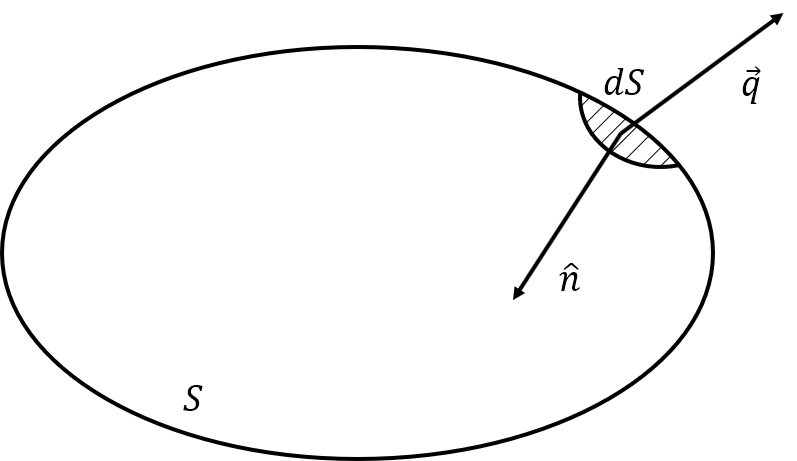
\includegraphics[scale=.75]{img/ass-1-1.1.png}
    \end{center}
    Let us consider a fixed closed surface $ S $ lying entirely in the fluid. If $ \hat{n} $ is a unit inward normal to the element $ \D S $, the rate at which mass flows into the surface through the boundary is 
    \begin{equation}
        \int_S \rho \vec{q}\hat{n}\D S \label{eq:1.1}
    \end{equation}
    The mass of fluid within the volume $ V $ enclosed by $ S $ is
    \begin{equation}
        \int_V \rho\D V\label{eq:1.2}
    \end{equation}
    Assuming that no fluid is created or annihilated within $ S $, the mass can only increase by flow through boundary.\\
    Equating the time rate of increase of the mass to \eqref{eq:1.1} we get,
    \[
        \frac{\partial}{\partial t}\int_V \rho\D V=\int_S \rho \vec{q}\hat{n}\D S=-\int_V \vec{\nabla}\left( \rho \vec{q} \right)\D V \text{[using Gauss's theorem]}
    \]
    Thus,
    \[
        \int_V\left\{ \frac{\partial \rho}{\partial t}+\vec{\nabla}\left( \rho \vec{q} \right)\right\}\D V =0
    \]
    Since the surface $ S $ can be replaced by any arbitrary closed surface drawn within it, we must have at every point,
    \[
        \frac{\partial \rho}{\partial t}+\vec{\nabla}\left( \rho \vec{q} \right)=0
    \]
    This is the equation of continuity for the motion of a compressible fluid.\\
    In the case of an incompressible fluid $ \frac{\partial \rho}{\partial t}=0 $. So,
    \[
        \vec{\nabla}\vec{q}=0
    \]
    In the case of irrotational motion, we have $ \vec{q}=-\vec{\nabla}\phi $ and therefore the equation of continuity for an incompressible liquid in irrotational motion becomes,
    \[
        \vec{\nabla}^2 \phi=0
    \]
\end{soln}
\newpage
\begin{prob}
    Derive the differential equation of streamline and path line. When do the streamline and path line coincides?
\end{prob}
\begin{soln}
    Let, $ \vec{q}=u\hat{i}+v\hat{j}+w\hat{k} $ be the velocity vector and $ \mathrm{d}\vec{r}=\hat{i}\mathrm{d}x+\hat{j}\mathrm{d}y+\hat{k}\mathrm{d}z $ be an infinitesimal arc-length of a fluid particle at point $ P $.\\
    
    A streamline is defined as a line which is everywhere parallel to the local velocity vector $ \vec{q} $.\\
    Since $ \mathrm{d}\vec{r} $ is parallel to $ \vec{V} $ we have,
    \begin{align*}
        & \mathrm{d}\vec{r}\times \vec{V}=0\\
        \Rightarrow & \begin{vmatrix}
            \hat{i}&\hat{j}&\hat{k}\\
            \mathrm{d}x&\mathrm{d}y&\mathrm{d}z\\
            u&v&w
        \end{vmatrix}=0\\
        \Rightarrow& \hat{i}(w\mathrm{d}y-v\mathrm{d}z)+\hat{j}(u\mathrm{d}z-w\mathrm{d}x)+\hat{k}(v\mathrm{d}x-u\mathrm{d}y)=0
    \end{align*}
    Separately setting each component to zero gives three differential equations which define the streamline.
    Now,
    \begin{align*}
        &\hat{i}(w\mathrm{d}y-v\mathrm{d}z)=0\\
        \Rightarrow& \frac{\mathrm{d}y}{v}=\frac{\mathrm{d}z}{w}\\
        &\\
        &\hat{j}(u\mathrm{d}z-w\mathrm{d}x)=0\\
        \Rightarrow& \frac{\mathrm{d}x}{u}=\frac{\mathrm{d}z}{w}\\
        &\\
        &\hat{k}(v\mathrm{d}x-u\mathrm{d}y)=0\\
        \Rightarrow& \frac{\mathrm{d}x}{u}=\frac{\mathrm{d}y}{v}
    \end{align*}
    So the differential equation of streamline is $ \frac{\mathrm{d}x}{u}=\frac{\mathrm{d}y}{v}=\frac{\mathrm{d}z}{w} $.\\

    \emph{Equation of path line}
    \begin{table}[H]
        \begin{minipage}{0.5\linewidth}
            \begin{align*}
                q&=\lim_{\delta t \to 0}\frac{\left( r+\delta r \right)-r}{\delta t}\\
                &=\lim_{\delta t \to 0}\frac{\delta r}{\delta t}\\
                &\\
                u\hat{i}+v\hat{j}+w\hat{k}&=\frac{\D q}{\D t}=\frac{\D x}{\D t}\hat{i}+\frac{\D y}{\D t}\hat{j}+\frac{\D z}{\D t}\hat{k}\\
                \Rightarrow& u=\frac{\D x}{\D t},\quad v=\frac{\D y}{\D t},\quad \text{ and } w=\frac{\D z}{\D t}
            \end{align*}
        \end{minipage}\hfill
        \begin{minipage}{0.45\linewidth}
            \centering
            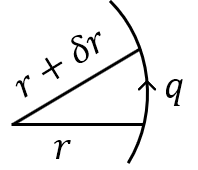
\includegraphics[scale=1]{img/ass-1-2.1.png}
        \end{minipage}
    \end{table}
    These are the differential equations of path line.\\

    Streamline and path line does coincide if the motion of the fluid is stationary. So when the partial derivative of the velocity vector $ (\vec{q}) $ with respect to time is zero then streamline and path line coincides. i.e., if $ \frac{\partial \vec{q}}{\partial t}=0 $ then streamline and path line coincides.
\end{soln}
\newpage
\begin{prob}
    State and proof Bernoulli's theorem for steady motion of an inviscid fluid. Hence, derive Bernoulli's theorem for barotropic flow.
\end{prob}
\begin{soln}
    
    \emph{Bernoulli's Theorem:} In the steady motion of an inviscid fluid the quantity $ \frac{p}{\rho}+k $ has the same value at every point of the same streamline, where $ p $ and $ \rho $ are the pressure and density, and $ k $ is the energy per unit mass of the fluid.
    \begin{proof}
        \hfill
        \begin{figure}[H]
            \centering
            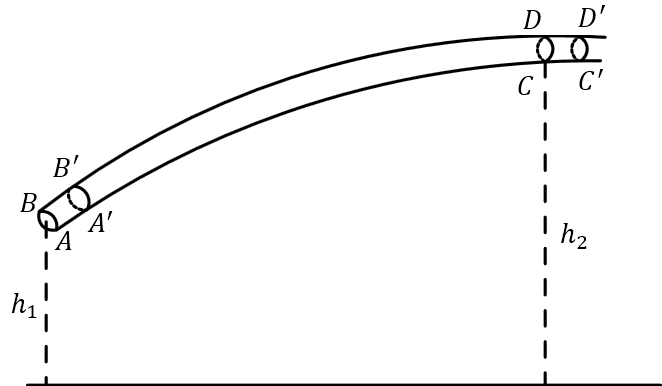
\includegraphics[scale=1]{img/ass-1-3.1.png}
        \end{figure}
        Consider a stream filament bounded by cross-sections $ AB,CD $ of areas $ \sigma_1 $ and $ \sigma_2 $ and let $ p_1,q_1,k_1 $ refer to values at $ AB $, while $ p_2,q_2,k_2 $ are the corresponding quantities at $ CD $.

        After a short time $ \delta t $ the fluid body $ ABCD $ will have moved to the position $ A'B'C'D' $ where
        \[AA'=q_1\delta t,\qquad CC'=q_2\delta T\]
        The mass $ m $ of the fluid between $ AB $ and $ A'B' $ or between $ CD $ and $ C'D' $ is 
        \[
            m=\sigma_1q_1\delta t \rho_1=\sigma_2q_2\delta t \rho_2
        \]
        The work done by the pressure thrusts in moving the fluid body from $ ABCD $ to $ A'B'C'D' $ is 
        \[
            p_1\sigma_1q_1\delta t-p_2\sigma_2q_2\delta t=m\left( \frac{p_1}{\rho_1}-\frac{p_2}{\rho_2} \right)
        \]
        Since the thrusts on the walls of filament, being perpendicular to the direction of motion, do no work.

        The gain of energy of the fluid body is $ mk_1-mk_2 $.\\
        Equating the work done to the gain of energy we get
        \[
            \frac{p_1}{\rho_1}+k_1=\frac{p_2}{\rho_2}+k_2
        \]
        which shows that $ \frac{p}{\rho}+k $ is constant along the streamline to which the stream filament shrinks when its cross-section tends to zero.
    \end{proof}
    \emph{Bernoulli's theorem for barotropic flow:}\\
    When the pressure is a function of the density the flow will be called \emph{barotropic}.

    Assuming steady barotropic flow and a conservative field of force for which the potential energy is $ \Omega $, the energy $ k $ per unit mass is $ k=\frac{1}{2}q^2+\Omega+E $, where $ E $ is the internal energy per unit and 
    \[ 
        E=\frac{p_0}{\rho_0}-\frac{p}{\rho} \int_{p_0}^p \frac{\D p}{\rho}
    \]
    Thus, Bernoulli's theorem becomes,
    \begin{align*}
        &\frac{p_1}{\rho_1}+\frac{1}{2}q_1^2+\Omega_1+\frac{p_0}{\rho_0}-\frac{p_1}{\rho_1}\int_{p_0}^{p_1}\frac{\D p}{\rho}=\frac{p_2}{\rho_2}+\frac{1}{2}q_2^2+\Omega_2+\frac{p_0}{\rho_0}-\frac{p_2}{\rho_2}\int_{p_0}^{p_2}\frac{\D p}{\rho}\\
        \Rightarrow & \int_{p_0}^{p_1}+\frac{\D p}{\rho}+\frac{1}{2}q_1^2+\Omega_1=\int_{p_0}^{p_2}+\frac{\D p}{\rho}+\frac{1}{2}q_2^2+\Omega_2\\
        \intertext{or,}
        &\int_{p_0}^{p}+\frac{\D p}{\rho}+\frac{1}{2}q^2+\Omega=\text{Constant along a streamline.}
    \end{align*}
    Hence, $ \int_{p_0}^{p}+\frac{\D p}{\rho}+\frac{1}{2}q^2+\Omega $ is Bernoulli's theorem for barotropic flow.
\end{soln}
\newpage
\begin{prob}
    Show that the variable ellipsoid 
    \[
        \frac{x^2}{a^2k^2t^4}+kt^2\left\{ \left( \frac{y}{b} \right)^2+\left( \frac{z}{c} \right)^2 \right\}=1,
    \]
    is a possible form of boundary surface of a liquid at any time $ t $.
\end{prob}
\begin{soln}
    \begin{equation}
        F(x,y,z,t)\equiv \frac{x^2}{a^2k^2t^4}+kt^2\left\{ \frac{y^2}{b^2} + \frac{z^2}{c^2} \right\}-1=0 \label{eq:4.1}
    \end{equation}
    The surface represented by \eqref{eq:4.1} will be a possible boundary surface if it satisfies the condition
    \begin{equation}
        \frac{\partial F}{\partial t}+u \pardx{F}+v\pardy{F}+w\pardz{F}=0\label{eq:4.2}
    \end{equation}
    where $ u,v,w $ are the velocity components, and they satisfy the equation of continuity
    \[
        \pardx{u}+\pardy{v}+\pardz{w}=0
    \]
    Now,
    \begin{align*}
        \frac{\partial F}{\partial t}&=\frac{\partial}{\partial t}\left\{ \frac{x^2}{a^2k^2t^4}+\frac{kt^2y^2}{b^2} + \frac{kt^2z^2}{c^2}-1 \right\}\\
        &=\frac{\partial}{\partial t}\frac{x^2}{a^2k^2t^4}+\frac{\partial}{\partial t}\frac{kt^2y^2}{b^2} +\frac{\partial}{\partial t} \frac{kt^2z^2}{c^2}-1 \\
        &=\frac{-4x^2}{a^2k^2t^5}+\frac{2tky^2}{b^2}+\frac{2tkz^2}{c^2}\\
        &=\frac{-4x^2}{a^2k^2t^5}+2kt\left(\frac{y^2}{b^2}+\frac{z^2}{c^2}\right)
    \end{align*}
    \begin{align*}
        \pardx{F}&=\pardx{}\left\{ \frac{x^2}{a^2k^2t^4}+kt^2\left( \frac{y^2}{b^2} + \frac{z^2}{c^2} \right)-1 \right\}\\
        &=\pardx{}\frac{x^2}{a^2k^2t^4}+\pardx{}kt^2\left( \frac{y^2}{b^2} + \frac{z^2}{c^2} \right)-\pardx{}1 \\
        &=\frac{2x}{a^2k^2t^4}
    \end{align*}
    \begin{align*}
        \pardy{F}&=\pardy{}\left\{ \frac{x^2}{a^2k^2t^4}+\frac{kt^2y^2}{b^2} + \frac{kt^2z^2}{c^2}-1 \right\}\\
        &=\pardy{}\frac{x^2}{a^2k^2t^4}+\pardy{}\frac{kt^2y^2}{b^2} +\pardy{} \frac{kt^2z^2}{c^2}-\pardy{}1\\
        &=\frac{2kt^2y}{b^2}
    \end{align*}
    \begin{align*}
        \pardz{F}&=\pardz{}\left\{ \frac{x^2}{a^2k^2t^4}+\frac{kt^2y^2}{b^2} + \frac{kt^2z^2}{c^2}-1 \right\}\\
        &=\pardz{}\frac{x^2}{a^2k^2t^4}+\pardz{}\frac{kt^2y^2}{b^2} +\pardz{} \frac{kt^2z^2}{c^2}-\pardz{}1\\
        &=\frac{2kt^2z}{c^2}
    \end{align*}
    Putting these values in \eqref{eq:4.2} we get,
    \begin{align*}
        & \frac{-4 x^2}{a^2 k^2t^5}+2kt\left( \frac{y^2}{b^2}+\frac{z^2}{c^2} \right)+u \frac{2x}{a^2k^2t^4}+v \frac{2kt^2y}{b^2}+w\frac{2kt^2z}{c^2}=0\\
        \Rightarrow & \left( u-\frac{2x}{t} \right)\frac{2x}{a^2k^2t^4}+\frac{2kty}{b^2}(y+vt)+\frac{2ktz}{c^2}(z+wt)=0
    \end{align*}
    If we accept $ u=\frac{2x}{t},v=-\frac{y}{t},w=-\frac{z}{t} $ the above equation is satisfied.\\
    Further
    \[
        \pardx{u}=\frac{2}{t}, \quad \pardy{v}=-\frac{1}{t},\quad \pardz{w}=-\frac{1}{t}
    \]
    $ \therefore $ Equation of continuity $ \pardx{u}+\pardy{v}+\pardz{w}=0 $ is also satisfied for $ \frac{2}{t}-\frac{1}{t}-\frac{1}{t}\equiv 0 $.\\
    Thus, $ \frac{x^2}{a^2k^2t^4}+kt^2\left\{ \frac{y^2}{b^2} + \frac{z^2}{c^2} \right\}=1$ is a possible boundary surface for a liquid with velocity components,
    \[
        u=\frac{2x}{t},v=-\frac{y}{t},w=-\frac{z}{t}
    \]
\end{soln}
\newpage
\begin{prob}
    Derive the equation of motion for incompressible inviscid fluid in the form $ \frac{\D\vec{q}}{\D t}=\vec{F}-\frac{1}{\rho}\vec{\nabla} p $.
\end{prob}
\begin{soln}
    \begin{figure}[H]
        \begin{center}
            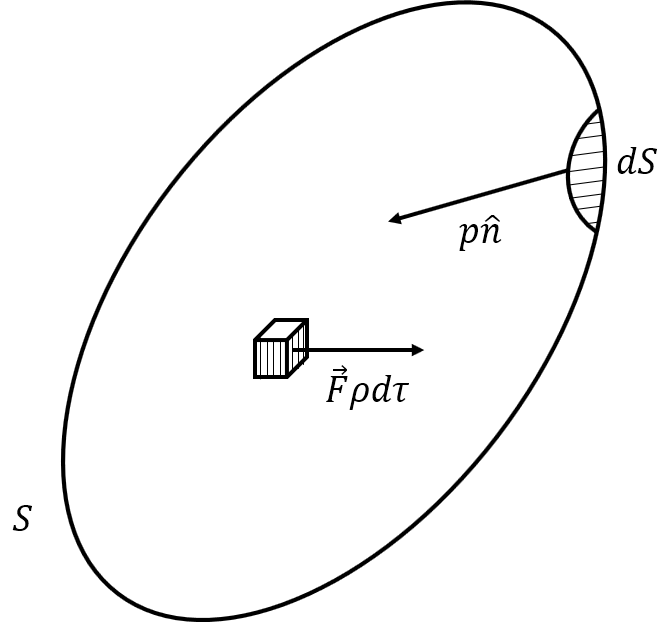
\includegraphics[scale=.75]{img/ass-1-5.1.png}
        \end{center}
    \end{figure}
    Let us consider the fluid body which at time $ t $ occupies the region interior to a closed surface $ S $. By the second law of motion, the total force acting in this fluid body is equal to the rate of change of linear momentum.\\
    The force is due to 
    \begin{enumerate}[label={\roman*)}]
        \item the normal pressure thrusts on the boundary,
        \item the external force (such as gravity), say $ \vec{F} $ per unit mass.
    \end{enumerate}
    Thus, the total force is,
    \[
        \int p\hat{n}\D S+\int \vec{F}\rho \D\tau=-\int(\vec{\nabla}p)\D\tau+\int \vec{F}\rho \D\tau\quad\text{ using Gauss's theorem}
    \]
    Equating this to the rate of change of linear momentum we get,
    \[
        \int\left( \vec{F}\rho-\vec{\nabla}p-\rho\frac{\D\vec{q}}{\D t} \right)\D V=0
    \]
    Since the shape of the fluid body and therefore the volume of integration is arbitrary we must have,
    \begin{align*}
        &\vec{F}\rho-\vec{\nabla}p-\rho\frac{\D\vec{q}}{\D t}=0\\
        \Rightarrow&\frac{\D\vec{q}}{\D t}=\vec{F}-\frac{1}{\rho}\vec{\nabla} p
    \end{align*}
    This is the equation of motion for incompressible fluid.
\end{soln}
\newpage
\begin{prob}
    Show that, $ u=\frac{-2xyz}{\left( x^2+y^2 \right)^2}, v=\frac{\left( x^2-y^2  \right)z}{\left( x^2+y^2 \right)^2} $ and $ w=\frac{y}{x^2+y^2} $ are the velocity components of a possible fluid motion. Is this motion irrotational?
\end{prob}
\begin{soln}
    We have,
    \[
        u=\frac{-2xyz}{\left( x^2+y^2 \right)^2},\quad v=\frac{\left( x^2-y^2  \right)z}{\left( x^2+y^2 \right)^2},\quad w=\frac{y}{x^2+y^2}
    \]
    Now,
    \begin{align*}
        \pardx{u}&=-2yz\left\{ \frac{1}{\left( x^2+y^2 \right)^2}\pardx{}x+x\pardx{}\frac{1}{\left( x^2+y^2 \right)^2} \right\}\\
        &=-2yz\left\{ \frac{1}{\left( x^2+y^2 \right)^2}-\frac{4x^2}{\left( x^2+y^2 \right)^3} \right\}\\
        &=-2yz\left\{ \frac{y^2-3x^3}{\left( x^2+y^2 \right)^3}\right\}\\
        &=2yz\left\{ \frac{3x^3-y^2}{\left( x^2+y^2 \right)^3}\right\}
    \end{align*}
    \begin{align*}
        \pardy{v}&=z\left\{ \frac{\left( x^2+y^2 \right)^2\left( -2y    \right)-\left( x^2-y^2 \right)2\left( x^2+y^2 \right)2y}{\left( x^2+y^2 \right)^4} \right\}\\
        &=z\left[ \frac{\left( x^2+y^2 \right)\left\{\left( x^2+y^2 \right)\left( -2y\right)-\left( x^2-y^2 \right)2(2y)\right\}}{\left( x^2+y^2 \right)^4} \right]\\
        &=z\left[ \frac{\left( x^2+y^2 \right)\left( -2y\right)-4y\left( x^2-y^2 \right)}{\left( x^2+y^2 \right)^3} \right]\\
        &=2yz\left[ \frac{ -x^2-y^2-2x^2+2y^2}{\left( x^2+y^2 \right)^3} \right]\\
        &=2yz\left[ \frac{y^2-3x^2}{\left( x^2+y^2 \right)^3} \right]\\
        &\\
        \pardz{w}&=0
    \end{align*}
    Now,
    \begin{align*}
        \pardx{u}+\pardy{v}+\pardz{w}&=-2yz\frac{3x^3-y^2}{\left( x^2+y^2 \right)^3}+2yz\frac{y^2-3x^2}{\left( x^2+y^2 \right)^3}+0\\
        &=0
    \end{align*}
    and hence the equation of continuity is fully satisfied. This shows that the motion is a possible one.\\
    Further the motion is irrotational, if,
    \[
        \pardz{v}-\pardy{w}=0,\quad\pardx{w}-\pardz{u}=0,\quad\text{ and }\pardy{u}-\pardx{v}=0
    \]
    Here,
    \begin{align*}
        \pardz{v}&=\frac{\left( x^2-y^2 \right)}{\left( x^2+y^2 \right)^2}
    \end{align*}
    \begin{align*}
        \pardy{w}&=\frac{1}{\left( x^2+y^2 \right)}+y\frac{-1}{\left( x^2+y^2 \right)^2}2y\\
        &=\frac{1}{x^2+y^2}-\frac{2y^2}{\left( x^2+y^2 \right)^2}\\
        &=\frac{x^2-y^2}{\left( x^2+y^2 \right)^2}\\
        &\\ 
        \therefore \pardz{v}-\pardy{w}&=\frac{\left( x^2-y^2 \right)}{\left( x^2+y^2 \right)^2}-\frac{x^2-y^2}{\left( x^2+y^2 \right)^2}\\
        &=0
    \end{align*}
    \begin{align*}
        \pardx{w}&=-\frac{2xy}{\left( x^2+y^2 \right)^2}\\
        &\\
        \pardz{u}&=-\frac{2xy}{\left( x^2+y^2 \right)^2}\\
        &\\
        \therefore \pardx{w}-\pardz{u}&=-\frac{2xy}{\left( x^2+y^2 \right)^2}+\frac{2xy}{\left( x^2+y^2 \right)^2}\\
        &=0
    \end{align*}
    \begin{align*}
        \pardy{u}&=-2xz\left\{ \frac{1}{\left( x^2+y^2 \right)^2}+y\frac{-2}{\left( x^2+y^2 \right)^3}2y \right\}\\
        &=-2xz\left\{ \frac{1}{\left( x^2+y^2 \right)^2}-\frac{4y^2}{\left( x^2+y^2 \right)^3} \right\}\\
        &=-2xz\left\{ \frac{x^2-3y^2}{\left( x^2+y^2 \right)^3} \right\}\\
        &\\
        \pardx{v}&=z\left\{ \frac{\left( x^2+y^2 \right)^2(2x)-\left( x^2-y^2 \right)2\left( x^2+y^2 \right)2x}{\left( x^2+y^2 \right)^4} \right\}\\
        &=z\left[ \frac{\left( x^2+y^2 \right)(2x)\left\{\left( x^2+y^2 \right)-2\left( x^2-y^2 \right)\right\}}{\left( x^2+y^2 \right)^4} \right]\\
        &=2xz\left[ \frac{x^2+y^2-2x^2+2y^2 }{\left( x^2+y^2 \right)^3} \right]\\
        &=2xz\left[ \frac{3y^2-x^2}{\left( x^2+y^2 \right)^3} \right]\\
        &\\
        \therefore \pardy{u}-\pardx{v}&=-2xz\left\{ \frac{x^2-3y^2}{\left( x^2+y^2 \right)^3} \right\}-2xz\left[ \frac{3y^2-x^2}{\left( x^2+y^2 \right)^3} \right]\\
        &=0
    \end{align*}
    Hence the motion is irrotational.
\end{soln}

\newpage
\begin{prob}
    Derive streaming motion past a circular cylinder.
\end{prob}
\begin{soln}
    Consider the stream whose complex potential is $ Uz $. If we insert the cylinder $ \abs{z}=a $ by the circle theorem, the complex potential becomes,
    \begin{equation}
        \label{eq:7.1}
        w=U\left( z+\frac{a^2}{z} \right)
    \end{equation}
    Which is therefore the complex potential of a circular cylinder placed in a stream whose velocity at infinity is $ U $ negatively along the x-axis.\\
    More generally, if we insert the cylinder in the uniform stream $ Uze^{-i\alpha} $, the complex potential by the circle theorem is,
    \[
        w=Uze^{-i\alpha}+\frac{Ua^2e^{i\alpha}}{z}
    \]
    If the center of the cylinder is at the point $ z_0 $, a simple change of origin yields the complex potential 
    \[
        w=Uze^{-i\alpha}+\frac{Ua^2e^{i\alpha}}{z-z_0}
    \]
    Returning to equation \eqref{eq:7.1}, since $ z=re^{i\theta} $ the stream function is,
    \[
        \psi=U\left( r\sin \theta-\frac{a^2}{r}\sin \theta \right)=Uy\left( 1-\frac{a^2}{r^2}\right)=\psi_1+\psi_2 
    \]
    where $ \psi_1=Uy, \,\psi_2=-\frac{a^2Uy}{x^2+y^2}  $\\
    Putting, $ \begin{aligned}[t]
        &\\
        \psi_1&=mUa\\
        \psi_2&=-nUa
    \end{aligned} $\\
    we get,
    \begin{align*}
        y&=ma\\
        x^2+\left( y-\frac{a}{2n} \right)^2&=\frac{a^2}{4n^2}
    \end{align*}
    So that the lines corresponding to $ \psi_1 $ and $ \psi_2 $ are straight lines parallel to the x-axis and circles touching at the x-axis at the origin.
\end{soln}
\newpage
\begin{prob}
    Define source, sink and doublet. Determine the complex potential foe a doublet of stream $ \mu $, placed at the point $ z=a $ which makes an angle $ \alpha $ with positive $ x- $axis.
\end{prob}
\begin{soln}
    
    \emph{Source:} If the two-dimensional motion of a liquid consists of outward radial flow from a point symmetrical in all directions in the reference plane, the point is called a simple source.\\
    \emph{Sink:} A sink is a negative source.\\
    Thus, a sink is a point of inward radial flow at which fluid is absorbed or annihilated continuously.\\
    \emph{Doublet:} A combination of a source of strength $ m $ and a sink of strength $ -m $ at a small distance $ \delta s $ apart such that $ m\delta s $ is finite is called a doublet.\\

    In the case of a source and equal sink, suppose that $ A $ and $ B$ are very close together, to that $ \alpha $ is small.\\Then,
    \begin{align*}
        w&=-m\log\left[ z\left( 1-\frac{ae^{i\alpha}}{z} \right) \right]+m\log\left[ z\left( 1+\frac{ae^{i\alpha}}{z} \right) \right]\\
        &=-m\log\left( 1-\frac{ae^{i\alpha}}{z} \right)+m\log\left( 1+\frac{ae^{i\alpha}}{z} \right)\\
        &=\frac{2mae^{i\alpha}}{z}+\frac{2ma^3e^{3i\alpha}}{3z^3}+\dots
    \end{align*}
    using the logarithmic series for the expansion of $ \log(1+k) $. Let $ 2ma=\mu $. Then,
    \[
        w=\frac{\mu e^{i\alpha}}{z}+\frac{\mu a^2 e^{3i\alpha}}{3z^3}+\dots
    \]
    Now let $ a\to 0, \mu $ remaining constant so that $ m\to\infty $. Then when $ A $ and $ B $ coincide, we get 
    \[
        w=\frac{\mu e^{i\alpha}}{z}
    \]
    This combination of an infinite source and sink at an infinitesimal distance apart is a doublet of strength $ \mu $.\\
    If the sink is situated at $ z=a $, then the complex potential is $ w=\frac{\mu e^{i\alpha}}{z-a} $.\\
    Hence, $ w=\frac{\mu e^{i\alpha}}{z-a} $ is the complex potential for a doublet of stream $ \mu $, placed at the point $ z=a $ which makes an angle $ \alpha $ with positive x-axis.
\end{soln}
\end{document}